\documentclass[11pt]{article}

% def commands for vars used in document
%-----------------------------------------------------------------
\newcommand{\myname}{Project 2}             
\newcommand{\course}{COMP 429}               
\newcommand{\assignment}{Varatep Buranintu\\John-Luke Laue}                  
\newcommand{\probs}{Jeffrey Limbacher}          
\newcommand{\duedate}{7 December 2014}              
%-----------------------------------------------------------------

% include latex packages
%-----------------------------------------------------------------
\usepackage{amsmath}            
\usepackage{amsthm}             
\usepackage{amssymb,latexsym}  
\usepackage{graphicx}          
\usepackage{verbatim}          
\usepackage{enumerate}          
\usepackage[left=1in,right=1in,top=0.75in,bottom=0.5in]{geometry} 
\usepackage[dvipsnames,usenames]{color}     
\usepackage{ifthen} 
\usepackage{tikz} 
\usetikzlibrary{automata,positioning} 
%-----------------------------------------------------------------

% def desired format for the title to appear on the first page
%-----------------------------------------------------------------
\newcommand{\mytitle}{
\begin{flushleft}
\bfseries
\assignment       \hspace*{\fill} \course \hspace*{\fill} \myname\\
\probs    \hspace*{\fill}                                 \duedate\\
\rule[10pt]{\linewidth}{1pt}
\end{flushleft}
}
%-----------------------------------------------------------------

% def desired page headings for all pages but first
%-----------------------------------------------------------------
\pagestyle{myheadings}
\markright{\course{} Varatep Buranintu, John-Luke Laue, Jeffrey Limbacher\ \ \ \ \ \ \ \ \ \ \ \ \ \ \ \myname}
%-----------------------------------------------------------------
 
 
%-----------------------------------------------------------------
\newenvironment{exercise}[2][Exercise]
 {\begin{trivlist}\item[\hspace{0pt} \textbf{#1}~\textbf{#2.}]}
 {\end{trivlist}}
%-----------------------------------------------------------------


%
% beg doc body
%-----------------------------------------------------------------
\begin{document}
\thispagestyle{empty}   % page 1: ignore page heading
\mytitle                

\renewcommand{\qedsymbol}{}

\section{Introduction and Environment Setup}
\ \ \ \ Our setup for the environment is a fresh install of Ubuntu 14.04 x64. There were no special libraries used in the making of the application. In order to run the program, the following steps should be taken:\begin{itemize}
\item Unzip the project ZIP folder to your desired location
\item Run $./build\_script.sh$ which will compile the program using gcc with all required parameters
\item Run the $proj.out$ executable using sudo along with arguments
\item If no arguments are given, the program will output the correct usage
\end{itemize}
A sample run:
\begin{itemize}
\item sudo $./project2.out\ 8.8.8.8\ 9876\ L\ 1100\ 6000\ 255\ 10\ 50$
\end{itemize}

\section{Challenges}
\ \ \ \ A big problem that we faced during this project was the issue of cross compatbility between operating systems. Varatep Buranintu was developing on OS X, John-Luke Laue on Linux 14.04, and Jeffrey Limbacher on Windows. This was due to a lack of consideration for compatibility on Linux and we encountered some issues with the \textit{udphdr} struct having more than one definition and there was ambiguity when switching the source files to a different operating system. 

\section{Correct Implementations}
\ \ \ \ 

\section{Problematic Implementations}
\ \ \ \ 

\section{Design Decisions}
\ \ \ \ The greatest design decision we had to conclude on was how to split the work up. For a project like this, modularity is key in developing a reusable codebase with independent segments in itself allowing multiple developers to work simultaneously on similar parts of the program without impeding each other's work. We agreed that the application would use multithreading in order to provide a seamless user experience and performance limiting possible gridlocks. The first thing we did was creating a header file called \textit{"includes.h"} that would import all of the required C standard libraries as well as act as the interface for our common program data. Such program data includes the Sender and Receiver functions \textit{sendto} and \textit{recvfrom} on the same socket. Another common program data used is the idea that both the Sender and Receiver need to be aware of the entropy type.  Our user arguments struct was also stored in the \textit{"includes.h"} file so that we would not have to re-declare or re-define it for every file in which it is used.
\begin{center}
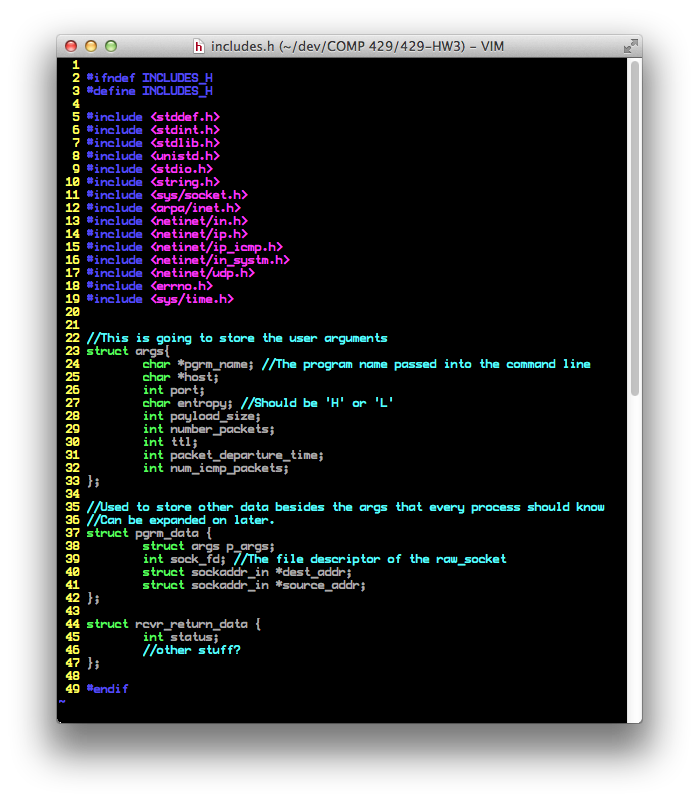
\includegraphics[scale=0.4]{images/includes-header.png}
\end{center}

\subsection{Sender}
\ \ \ \ We designated the Sender to stay on the main thread as this is the core of our project that requires the most attention from the operating system. The sender is broken up into two categories: send functions \textit{("sender.c")} and fill-out functions \textit{("network.c")}. \\
\begin{center}
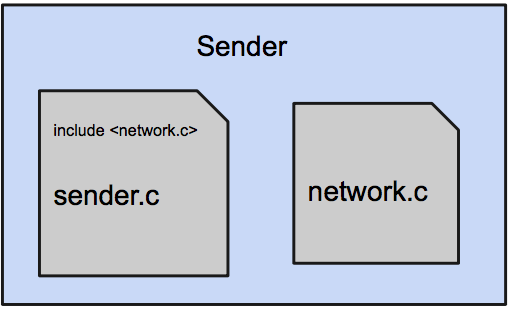
\includegraphics[scale=0.3]{images/sender-design.png}
\end{center}

\subsection{Receiver}
\ \ \ \ John-Luke Laue intended the Receiver to have the same design as the Sender, although he quickly realized that this was unnecessary as a result of unpacking not requiring a multitude of functions in order to work properly.
\begin{center}
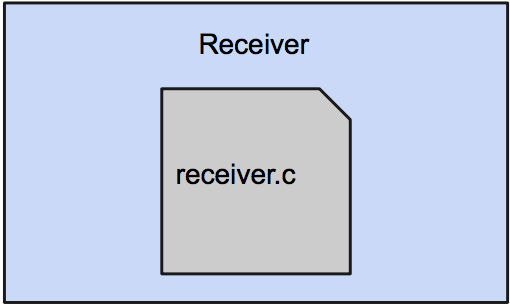
\includegraphics[scale=0.3]{images/receiver-design.png}
\end{center}

\section{Project Hindsight}
\ \ \ \ 

\section{Allocation of Work}
\ \ \ \ The collaborators of project collectively decided on how the work would be split up. The individuals of the team came up with different designs for the task, but we conjointly decided to capitalize on Jeffrey Limbacher's well-thought architecture. Upon general completion of the architecture design, we realized the significance of modularity in this project. Since there are two main hubs (the sender and the receiver) in this project, it made sense to assign at least one person per hub. John-Luke Laue was assigned the task of bringing together the receiver by himself, since this part was relatively straightforward. Varatep Buranintu and Jeffrey Limbacher modularly designed the sender hub and pooled resources together. Varatep Buranintu was responsible for the ICMP (head and tails) segment whilst Jeffrey Limbacher developed the UDP segment. Jeffrey Limbacher also built the raw socket and IP header as his tasks. Varatep Buranintu generated the project documentation and ensured the source code documentation (comments) is superlative so that another developer would be able to pick up where the project was left off.

\end{document}
